% Informe técnico: cinemática y modelo 3D del brazo XK-JS1-1 (II-2026)
% Basado en global/plantillas/plantilla_informe.tex
% Compilar desde esta carpeta:  latexmk -pdf informe_cinematica_modelo_3d.tex
\documentclass[a4paper,12pt]{article}

%*** TAMAÑO DE PAPEL ***
\usepackage{geometry}
\geometry{letterpaper, margin=2.5cm}
\usepackage{setspace}
\usepackage{titlesec}

%*** IDIOMA
\usepackage[spanish, es-nodecimaldot, mexico]{babel}
\usepackage[utf8]{inputenc}
% *** fuente***
\usepackage[light,condensed,math]{kurier}
\usepackage[T1]{fontenc}

% *** color ***
\usepackage[table]{xcolor}
\definecolor{verde}{RGB}{80,180,60}
\definecolor{rojo}{rgb}{1,0.36,0.24}
\definecolor{gray}{RGB}{242,242,242}
\definecolor{cafe}{RGB}{128,64,0}
\definecolor{grayblack}{RGB}{50,50,50}
\definecolor{naranja}{RGB}{194,98,12}

%*** FIGURAS***
\usepackage{graphicx}
\graphicspath{{figuras/}}
\usepackage{float}
\usepackage{subcaption}
\usepackage{tikz}
\usepackage{textcomp}

%*** tablas ***
\usepackage{booktabs}
\usepackage{colortbl}
\usepackage{longtable}
\usepackage{array}

%***referencias***
\usepackage{hyperref}
\hypersetup{colorlinks=true, linkcolor=blue, urlcolor=blue}

%***ECUACIONES***
\usepackage{mathtools}
\usepackage{amssymb}

% *** ENCABEZADO***
\usepackage{lastpage}
\usepackage{fancyhdr}
\pagestyle{fancy}

%*******CODIGOS***
\usepackage{listings}
\lstset{
  basicstyle=\ttfamily\small, frame=single, breaklines=true,
  postbreak=\mbox{$\hookrightarrow$}, captionpos=b, numbers=none,
  keywordstyle=\color{naranja}, commentstyle=\color{gray!60!black}, columns=fullflexible
}

\renewcommand{\headrulewidth}{0.6pt}
\let\oldheadrule\headrule
\renewcommand{\headrule}{\color{cafe}\oldheadrule}
\renewcommand{\footrulewidth}{0.6pt}
\let\oldfootrule\footrule
\renewcommand{\footrule}{\color{cafe}\oldfootrule}

% PIE DE PAGINA
\newcommand{\titulo}{\small{CINEMÁTICA Y MODELO 3D}}
\cfoot{\textcolor{black}{\small{\titulo}}}
\lfoot{}
\rfoot{\textcolor{black}{\small Pag. \thepage\ - \pageref{LastPage}}}

% ENCABEZADO
\newcommand{\institucion}{UMSA}
\newcommand{\tema}{GEMELO DIGITAL GEOMÉTRICO}
\lhead{\textcolor{black}{ETN-902, ETN-1034, ETN-1000}}
\chead{\textcolor{black}{\tema}}
\rhead{\textcolor{black}{\institucion}}
\setlength{\headheight}{15pt}
\titleformat{\section}{\color{cafe}\normalfont\Large\bfseries}{\thesection}{1em}{}
\titleformat{\subsection}{\color{cafe}\normalfont\large\bfseries}{\thesubsection}{1em}{}

% Marca de supuestos
\newcommand{\supuesto}{\textcolor{naranja}{\textsc{supuesto}}}
\newcommand{\codigo}[1]{\texttt{\small #1}}

\begin{document}
\color{grayblack}

%==================================================================== CARÁTULA
\begin{titlepage}
\thispagestyle{empty}
% Si existe la imagen de fondo de los informes anteriores, se usa
\IfFileExists{portada.pdf}{%
\begin{tikzpicture}[remember picture,overlay]
  \node [inner sep=0pt] at (current page.center) {\includegraphics[width=21cm]{portada.pdf}};
\end{tikzpicture}}{}

\vspace*{1.5cm}
\begin{center}
{\large \bfseries UNIVERSIDAD MAYOR DE SAN ANDRÉS}\\[0.1cm]
{\normalsize Facultad de Ingeniería -- Carrera de Ingeniería Electrónica}\\[1cm]

{\color{cafe}\rule{\textwidth}{0.8pt}}\\[0.3cm]
{\LARGE \bfseries CINEMÁTICA Y MODELO 3D DEL BRAZO}\\[0.3cm]
{\large Levantamiento de medidas, cinemática directa e inversa, relación pulsos--movimiento,\\
espacio de trabajo y gemelo digital geométrico}\\[0.3cm]
{\normalsize Brazo Robótico de 4 Grados de Libertad (XK-JS1-1)}\\
{\color{cafe}\rule{\textwidth}{0.8pt}}\\[0.8cm]

{\normalsize \bfseries Asignaturas concurrentes:}\\[0.1cm]
Sistemas de Control II (ETN-902)\\
Aplicación de Técnicas de Control (ETN-1034)\\
Bases de Datos (ETN-1000)\\[0.4cm]
Complemento del Laboratorio Integrado N.º 5 (Fase 2: gemelos digitales)\\[0.8cm]
\end{center}

\begin{tabular}{@{}ll}
\textbf{Docente:} & Ing. Jorge Antonio Nava Amador\\
\textbf{Auxiliares de docencia:} & Limber Ajnota -- Fabián Plata -- Franz Choque\\
\textbf{Repositorio:} & \url{https://github.com/GabAndGom/Brazo-de-4-grados-de-libertad}\\
\textbf{Página:} & \url{https://brazo-4gdl.pages.dev}\\
\end{tabular}

\vspace{0.8cm}
\begin{minipage}[t]{0.55\textwidth}
\textbf{Equipo de Control (ETN-902 / ETN-1034):}
\begin{itemize}\setlength\itemsep{0pt}
\item Gabriel Andrés Gómez Calla
\item José Lenin Mamani Choque
\item Miguel Alejandro Lima Huarachi
\item Román Abner Machicado Arequipa
\end{itemize}
\end{minipage}\hfill
\begin{minipage}[t]{0.42\textwidth}
\textbf{Equipo de Cómputo (ETN-1000):}
\begin{itemize}\setlength\itemsep{0pt}
\item Miguel Alejandro Lima Huarachi
\item Marco Eduardo Chura Rondo
\end{itemize}
\end{minipage}

\vfill
\begin{center}
La Paz, Bolivia -- Octubre de 2026 -- Gestión II/2026
\end{center}
\end{titlepage}
\normalcolor

\tableofcontents
\newpage

%==================================================================== 1
\section{Introducción}

El brazo XK-JS1-1 del Laboratorio de Control se ha documentado hasta ahora como un manipulador de tres
``ejes'' (X, Y y Z) más una garra. La auditoría de la Fase 1 identificó su hardware, sus variables y su
lazo abierto con supervisión discreta, pero no estableció la relación geométrica entre los pulsos que emite
el PLC y la posición de la garra. Esa relación no es directa: el brazo \textbf{no es cartesiano}. Los
husillos X e Y accionan un mecanismo de bielas que lleva la garra, y la posición de la garra hay que
calcularla resolviendo ese mecanismo.

Este informe desarrolla esa geometría. Se toman como base los bocetos acotados y las fotos etiquetadas de la
planta del 20 de octubre de 2026, el manual de fábrica y los informes anteriores. A partir de ellos se
obtienen la estructura cinemática, la cinemática directa e inversa, el jacobiano, la relación
motor--articulación y el espacio de trabajo. Con los mismos parámetros se construye un modelo 3D articulado,
que se integra en la página del proyecto como un gemelo digital geométrico controlable desde el navegador.

\subsection{Relación con la guía vigente}
La Guía de Laboratorio N.º 5 (semanas 9 a 13) pide gemelos digitales de las plantas, su contraste con datos
reales y el análisis de controlabilidad y observabilidad en MATLAB/Simulink. Este trabajo aporta la
\textbf{parte geométrica} del gemelo del brazo: sin la cinemática no se puede pasar de pulsos a posición
de la garra. No reemplaza la identificación dinámica ni el modelo en espacio de estados de los Laboratorios 4
y 5. La sección~\ref{sec:guia} detalla qué entregables cubre.

%==================================================================== 2
\section{Objetivos}
\subsection{Objetivo general}
Obtener el modelo cinemático del brazo XK-JS1-1 a partir de sus medidas reales y construir con él un modelo
3D articulado, controlable desde la página web del proyecto, que exprese los movimientos en pulsos del PLC.

\subsection{Objetivos específicos}
\begin{itemize}
\item Levantar las medidas de cada pieza y deducir la estructura cinemática y sus grados de libertad.
\item Deducir la cinemática directa e inversa, incluido el cierre del lazo de bielas, las múltiples
      soluciones y los límites de recorrido.
\item Calcular el jacobiano, las singularidades y el ángulo de transmisión del mecanismo.
\item Establecer la relación pulsos $\rightarrow$ movimiento de cada eje y señalar las restricciones de la CPU 224.
\item Obtener el espacio de trabajo y validar las implementaciones entre sí y frente al modelo 3D.
\item Integrar el modelo 3D y la cinemática en la página, con una interfaz preparada para el PLC real.
\end{itemize}

\subsection{Alcance y supuestos}
El trabajo se hizo en gabinete y no se movieron los actuadores. Las cotas que no se pudieron medir
(posición de algunos pivotes, paso del husillo, micropasos de los drivers y reducción de la base) se
marcan como \supuesto{} en este informe, en el código y en la página. Todas están en un solo archivo
(\codigo{web/js/cinematica.js}): cuando se midan en la planta, basta corregirlas ahí y volver a generar las
figuras y el modelo.

%==================================================================== 3
\section{Marco teórico}

\subsection{Cinemática directa e inversa}
La cinemática directa obtiene la posición del efector final a partir de las variables articulares. La
inversa resuelve el problema contrario: qué variables articulares llevan el efector a una posición dada.
La directa tiene una sola solución, mientras que la inversa puede tener varias soluciones o ninguna
\cite{craig,spong}.

\subsection{Mecanismos de lazo cerrado}
Cuando los eslabones forman un lazo cerrado, no todas las articulaciones son independientes: los ángulos de
las articulaciones pasivas se obtienen imponiendo que el lazo se cierre. En el mecanismo biela--manivela
invertido que se estudia aquí, la ecuación de cierre es una distancia constante entre dos pivotes y se
resuelve con la ley de cosenos \cite{norton}.

\subsection{Movilidad de Grübler--Kutzbach}
Para un mecanismo plano con $n$ eslabones (incluido el fijo), $j_1$ pares de un grado de libertad y $j_2$
pares de dos, la movilidad es
\begin{equation}
M = 3(n-1) - 2j_1 - j_2 .
\end{equation}

\subsection{Jacobiano y singularidades}
El jacobiano $J = \partial \mathbf{x}/\partial \mathbf{q}$ relaciona velocidades articulares con velocidades
del efector. Donde $\det J = 0$ el manipulador pierde una dirección de movimiento (singularidad). En un
mecanismo de bielas, además, el \emph{ángulo de transmisión} entre la biela y el eslabón que acciona indica
la calidad de la transmisión de fuerza. Conviene que se mantenga entre unos 40° y 140° \cite{norton}.

\subsection{Motores paso a paso, husillos y tren de pulsos}
Un motor de 1.8° por paso da 200 pasos por vuelta. El driver subdivide cada paso en $\mu$ micropasos, de
modo que el motor necesita $200\mu$ pulsos por vuelta. Un husillo de paso $p$ avanza $p$ milímetros por
vuelta. Como no hay encoders, la posición se estima contando pulsos desde una referencia (homing):
$q_{est} = q_0 + N_p\,\Delta q$. La CPU 224 genera trenes de pulsos (PTO) por hardware solo en Q0.0 y Q0.1,
hasta 20~kHz \cite{s7200}.

%==================================================================== 4
\section{Levantamiento de medidas}

\subsection{Método}
Se contó con 20 fotografías de la planta. Una parte son bocetos a mano con cotas en centímetros, cada pieza
numerada. La otra son fotos del brazo con etiquetas que llevan esos mismos números. Cruzando ambas se
identificó cada pieza y su función. El detalle está en
\codigo{semestres/2026\_II/modelo-3d/levantamiento/levantamiento\_medidas.md}. Cada dato se clasificó como
\emph{leído} (cota del boceto), \emph{estimado} (medido sobre la foto con una cota leída como escala),
\emph{fabricante} (manual o ficha comercial) o \supuesto. Las cotas estimadas del mecanismo se
ajustaron con la foto de perfil del manual (figura 1.3.3 A): con ellas el modelo reproduce la pose de esa
foto con menos de 5 mm de diferencia en los pivotes $B$ y $C$. No se encontraron fotos ni planos públicos
del equipo; la única referencia externa es la ficha comercial del fabricante \cite{ficha}.

\subsection{Funcionamiento deducido}
\begin{enumerate}
\item La \textbf{base giratoria} (disco superior 11, columna 7 y bloque 2) gira sobre el disco inferior. El
      motor NEMA 17 va montado sobre ella y la acciona con engranajes, según el manual.
\item El \textbf{bloque 2} está atornillado a la columna y lleva la tuerca del husillo inferior. Al girar
      ese husillo, \textbf{todo el bastidor} (placas 5 y 10, cuatro guías 16, los dos husillos y los dos NEMA 23)
      se desliza a través del bloque 2. Esto es el \textbf{carro X}.
\item El \textbf{bloque 1} lleva la tuerca del husillo superior y corre sobre el bastidor. Esto es el
      \textbf{carro Y}: su carrera es relativa al bastidor.
\item Sobre el bloque 1, la escuadra 6 sostiene el pivote $C$ de la \textbf{biela 12}, que empuja el vértice
      $B$ de la escuadra 8. La escuadra 8 está fija al \textbf{brazo 9} y forma con él un balancín que
      pivota en $A$, sobre la placa delantera 5.
\item La \textbf{varilla 13} y los dos \textbf{postes 14} forman con el brazo 9 un paralelogramo que mantiene
      la pinza siempre horizontal. Están en el plano central del brazo: la varilla pasa entre las dos placas
      de la escuadra 8, y los postes van al centro de la placa 5 y al centro de la pinza.
\item Los finales de carrera van en barras sobre las placas 5 y 10. En cada barra, el de arriba toca el
      bloque 1 y el de abajo el bloque 2: son dos por eje, como indica el manual.
\end{enumerate}
Esta interpretación coincide con el manual de fábrica, que describe el eje X como ``adelante--atrás'' y el
eje Y como ``arriba--abajo'' \cite{manual}, y con el GLB de trabajo, cuyos nodos se llaman
\emph{CarroHorizontal} y \emph{CarroElevacion}.

\subsection{Tabla de piezas}
\begin{longtable}{@{}p{0.6cm}p{3.6cm}p{5.2cm}p{2.0cm}p{2.6cm}@{}}
\toprule
\textbf{N.º} & \textbf{Pieza} & \textbf{Cotas [mm]} & \textbf{Estado} & \textbf{Unión}\\
\midrule\endhead
11 & Discos de base & Ø165 × 15 (×2); hueco Ø42 & leída & sup.: revoluta $\theta$\\
7 & Columna en H & 120 × 100 × 71 & leída & fija\\
2 & Bloque fijo (tuerca X) & 100 × 130 × 40; bujes Ø28, tuerca Ø50 & leída & fija\\
5, 10 & Placas del bastidor & 120 ancho × 110 alto × 13 & leída & fijas al bastidor\\
16 & Guías ×4 & Ø16 × 300; a $\pm$37.5 del husillo & leída & fijas al bastidor\\
3 & Adaptadores NEMA 23 ×2 & 57 × 57 × 50 & leída & fijos a la placa 10\\
-- & Bastidor (carro X) & -- & -- & \textbf{prismática} $s_X$\\
1 & Bloque del carro Y & 100 × 130 × 50 & leída & \textbf{prismática} $s_Y$\\
6 & Escuadra (pivote $C$) & 110 alto, base 49, punta 24, esp. 11 & leída & fija al bloque 1\\
12 & Biela & 240 × 24 × 11.1; ranura 160 & leída & revoluta $C$, $B$\\
8 & Escuadra del balancín & igual que 6 & leída & fija al brazo 9\\
9 & Brazo principal & ancho 46, esp. 10; largo A--E \supuesto{} 300 & leída / est. & revoluta $A$\\
13 & Varilla & Ø11 × 300 & leída & revolutas $A'$, $E'$\\
14 & Postes ×2 & 46 × 10 & leída & fijos\\
4 & Cuerpo de la pinza & 80 × 55 × 55 & leída & revoluta $E$\\
15 & Mordazas & 150 × 80 × 30 (por confirmar) & leída & garra ON/OFF\\
17 & Horquilla en U & 55.4 × 49.7 × 25.4 & leída & ¿pivote $A$?\\
18 & Soporte & 28.3 × 30 × 13.9 & leída & ubicación por confirmar\\
\bottomrule
\caption{Piezas del brazo (resumen). Bocetos en cm, pasados a mm.}
\end{longtable}

\subsection{Parámetros cinemáticos}
\begin{table}[H]
\centering
\begin{tabular}{@{}llll@{}}
\toprule
\textbf{Símbolo} & \textbf{Descripción} & \textbf{Valor} & \textbf{Origen}\\
\midrule
$L_{12}$ & distancia entre pivotes $C$--$B$ de la biela & 235 mm & estimado (boceto: 24 cm total)\\
$a$ & distancia $A$--$B$ del balancín & 145 mm & estimado (foto del manual)\\
$\beta$ & ángulo entre $A$--$B$ y el brazo & 50° & estimado (foto del manual)\\
$L_9$ & distancia $A$--$E$ del brazo & 300 mm & igual a la varilla 13\\
$L_{14}$ & postes del paralelogramo (entre pivotes) & 70 mm & estimado (poste de 46 + soporte)\\
$u_{50}$ & placa 5 con $s_X=0$ (desde el eje $\theta$) & 52 mm & bloque 2 + holgura\\
$u_A$, $h_A$ & pivote $A$ (desde la placa 5; sobre la mesa) & 20 mm; 236 mm & estimado (foto)\\
$c_{u0}$, $c_h$ & pivote $C$ respecto de $A$ con $s_Y=0$ & $-252$ mm; 125 mm & derivado\\
$d_g$, $h_g$ & TCP respecto del pivote $E$ & 135 mm; 20 mm & estimado (foto)\\
$s_X$ & recorrido útil del carro X & 0--120 mm & \supuesto{} (ficha del fabricante)\\
$s_Y$ & recorrido útil del carro Y & 0--170 mm & \supuesto{} (300 $-$ 2·13 $-$ 100 $-$ 2·2)\\
$\theta$ & rango de la base & $\pm$175° & \supuesto{} (manual: 360°)\\
\bottomrule
\end{tabular}
\caption{Parámetros del modelo cinemático.}
\label{tab:parametros}
\end{table}

%==================================================================== 5
\section{Esquema cinemático y grados de libertad}

\begin{figure}[H]
\centering
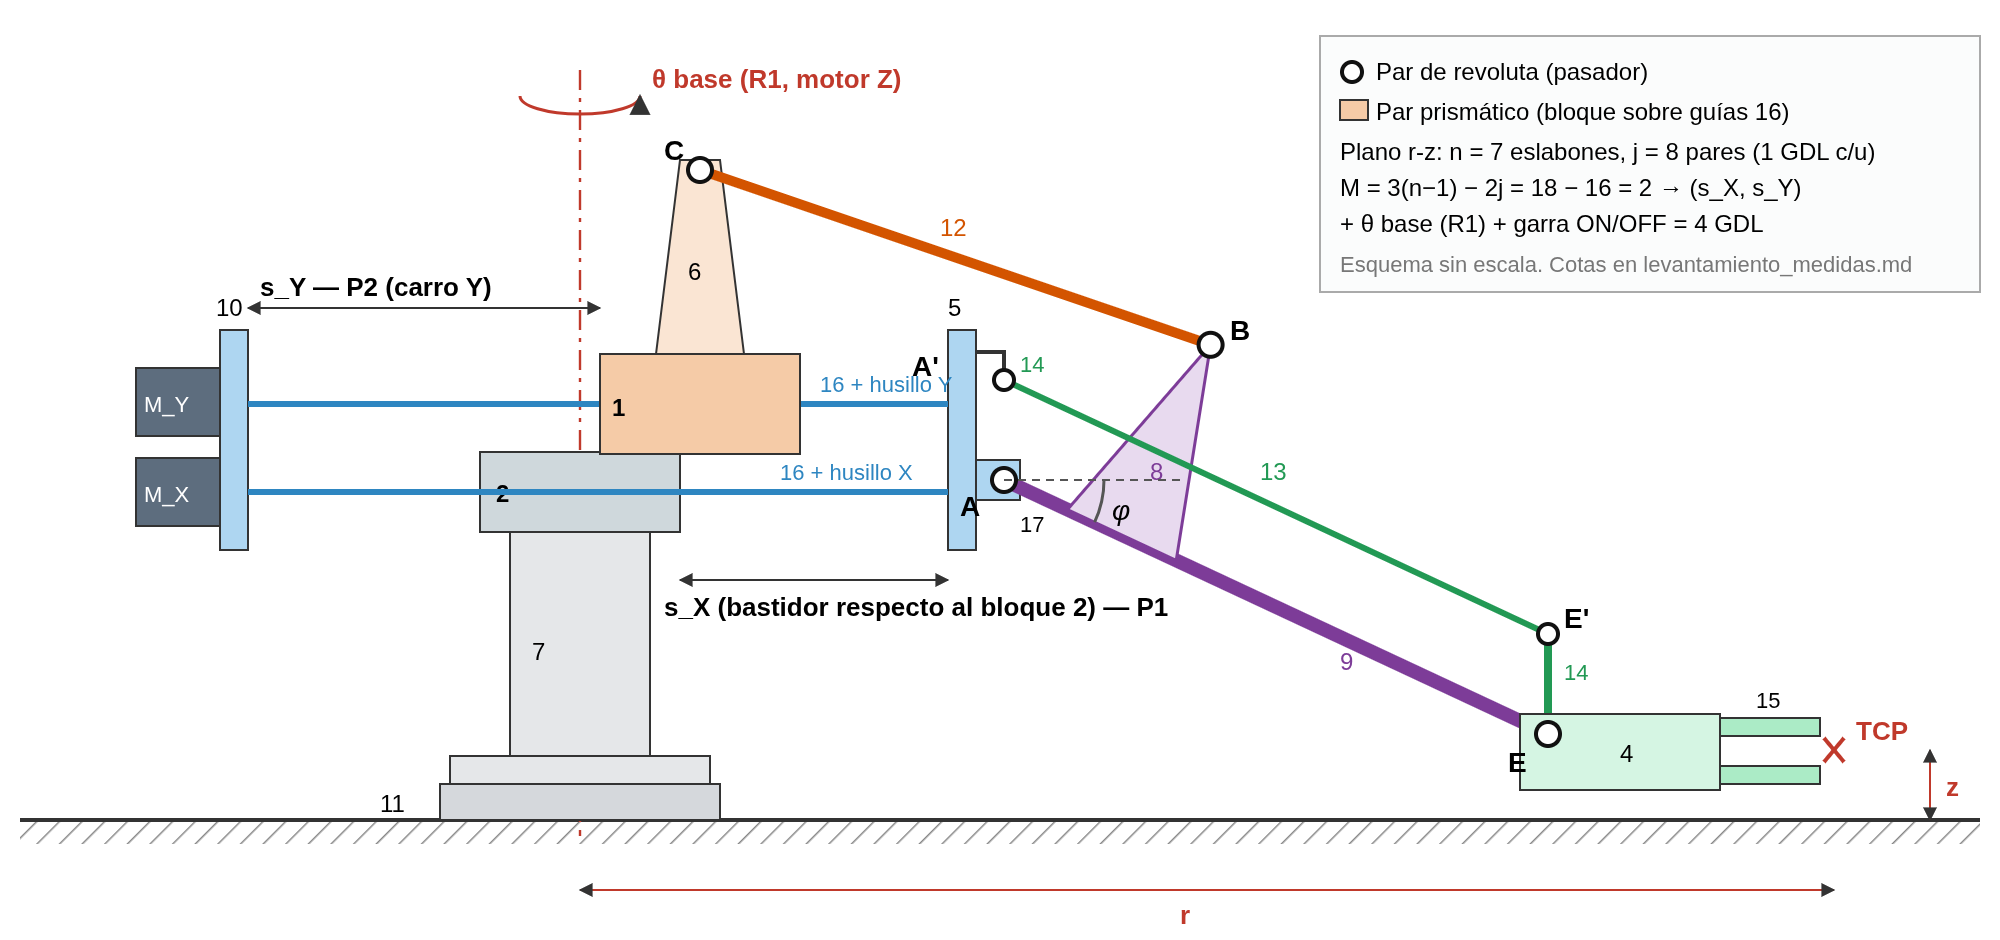
\includegraphics[width=\textwidth]{esquema_cinematico.png}
\caption{Esquema cinemático en el plano $r$--$z$. Pares de revoluta ($\circ$), pares prismáticos (bloques
sobre guías) y pivotes $A$, $A'$, $B$, $C$, $E$, $E'$.}
\label{fig:esquema}
\end{figure}

En el plano del brazo intervienen siete eslabones: (1) base giratoria con columna y bloque 2, (2) bastidor,
(3) bloque 1 con escuadra 6, (4) biela 12, (5) balancín 9+8, (6) varilla 13 y (7) pinza. Hay ocho pares de
un grado de libertad: dos prismáticos ($s_X$ entre 1 y 2, $s_Y$ entre 2 y 3) y seis revolutas ($C$, $B$,
$A$, $E$, $A'$, $E'$). Entonces
\begin{equation}
M = 3(7-1) - 2\cdot 8 = 2 .
\end{equation}
Las dos coordenadas independientes son $s_X$ y $s_Y$. Sumando el giro de la base ($\theta$) y la garra
ON/OFF, el equipo tiene los \textbf{4 GDL} de su nombre. La garra no cambia la posición del TCP. El
paralelogramo no agrega movilidad: solo fija la orientación de la pinza.

%==================================================================== 6
\section{Cinemática directa}

\textbf{Variables articulares:} $\mathbf{q} = (\theta, s_X, s_Y)$ y el estado de la garra $g \in \{0,1\}$.
\textbf{Salida:} posición del TCP en coordenadas cilíndricas $(\theta, r, z)$ y cartesianas $(X, Y, Z)$.
El origen está en el eje de giro, a nivel de la mesa, con $X$ hacia el sensor inductivo ($\theta = 0$) y
$Z$ hacia arriba.

\paragraph{Paso 1: posición de los pivotes en el bastidor.} Con $A$ como origen,
\begin{equation}
\mathbf{C}-\mathbf{A} = \begin{bmatrix} s_Y + c_{u0}\\ c_h\end{bmatrix},\qquad
\mathbf{B}-\mathbf{A} = a\begin{bmatrix}\cos\psi\\ \sin\psi\end{bmatrix}.
\end{equation}
La posición de $C$ respecto de $A$ \textbf{no depende de} $s_X$, porque el bloque 1 y el pivote $A$ viajan
juntos con el bastidor.

\paragraph{Paso 2: cierre del lazo $A$--$B$--$C$.} La biela es rígida: $|\mathbf{B}-\mathbf{C}| = L_{12}$.
En el triángulo $A B C$ se conocen los tres lados, $a$, $L_{12}$ y $d = |\mathbf{C}-\mathbf{A}|$. Por la
ley de cosenos, el ángulo $\gamma$ en $A$ es
\begin{equation}
d = \sqrt{(s_Y+c_{u0})^2 + c_h^2},\qquad \cos\gamma = \frac{a^2 + d^2 - L_{12}^2}{2ad},
\end{equation}
y el ángulo de $A$--$B$ resulta
\begin{equation}
\psi = \operatorname{atan2}(c_h,\, s_Y + c_{u0}) - \gamma .
\label{eq:psi}
\end{equation}
El signo menos elige la \emph{rama de montaje} real, con $B$ por debajo de la recta $A$--$C$, como en las
fotos. El lazo cierra solo si $|a-L_{12}| \le d \le a+L_{12}$, es decir, $90 \le d \le 380$ mm. Dentro del
recorrido $d$ varía entre 150 y 281 mm, así que el lazo siempre cierra.

\paragraph{Paso 3: ángulo del brazo.} La escuadra 8 está fija al brazo con un ángulo $\beta$:
\begin{equation}
\varphi = \psi - \beta .
\end{equation}

\paragraph{Paso 4: posición de la garra.} El pivote $E$ está en el extremo del brazo, y el paralelogramo
mantiene la pinza horizontal, por lo que el TCP está a una distancia fija $(d_g, -h_g)$ de $E$:
\begin{align}
r &= u_{50} + s_X + u_A + L_9\cos\varphi + d_g, \label{eq:r}\\
z &= h_A + L_9\sin\varphi - h_g, \label{eq:z}\\
X &= r\cos\theta,\quad Y = r\sin\theta,\quad Z = z .
\end{align}
El carro X aparece \emph{solo} en $r$: es una traslación radial pura. El carro Y entra a través de
$\varphi(s_Y)$ y mueve la garra sobre un arco de radio $L_9$, cambiando a la vez $r$ y $z$.

\begin{figure}[H]
\centering
\begin{subfigure}{0.49\textwidth}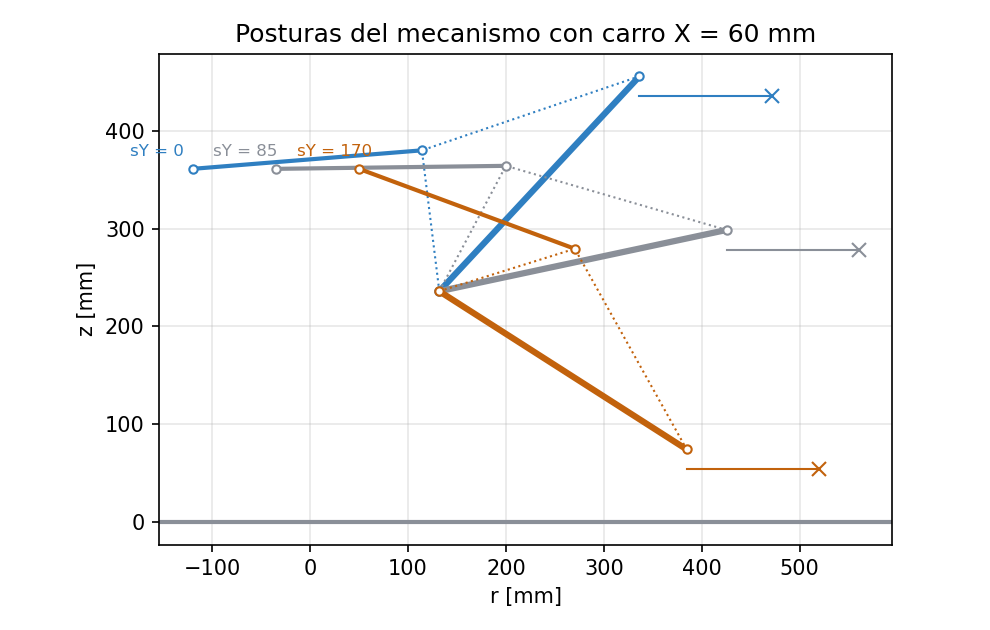
\includegraphics[width=\textwidth]{posturas_mecanismo.png}
\caption{Posturas del mecanismo para tres valores de $s_Y$.}\end{subfigure}
\begin{subfigure}{0.49\textwidth}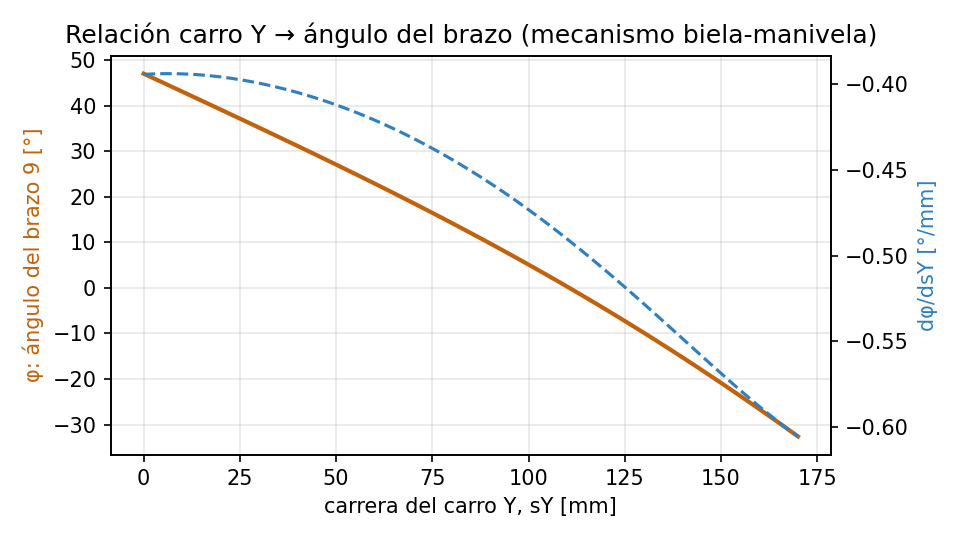
\includegraphics[width=\textwidth]{phi_vs_carro_y.png}
\caption{$\varphi(s_Y)$ y su derivada.}\end{subfigure}
\caption{Relación carro Y $\rightarrow$ ángulo del brazo.}
\label{fig:phi}
\end{figure}

Con los parámetros de la tabla~\ref{tab:parametros}, $\varphi$ va de $47.0°$ ($s_Y=0$, brazo arriba) a
$-32.6°$ ($s_Y = 170$ mm, brazo abajo), con $d\varphi/ds_Y \approx -0.45$ °/mm casi constante.

%==================================================================== 7
\section{Cinemática inversa}

Dado un objetivo $(X, Y, Z)$ se procede así:

\paragraph{Base.}
\begin{equation}
r = \sqrt{X^2+Y^2},\qquad \theta = \operatorname{atan2}(Y,X) + k\cdot 360°,\quad k\in\{-1,0,1\}.
\end{equation}
Se conservan los valores de $\theta$ que caen en $[\theta_{min}, \theta_{max}]$ y se elige el más cercano
a la posición actual, para que la base no dé una vuelta innecesaria. Si $r \approx 0$ el objetivo está
sobre el eje de giro y se rechaza.

\paragraph{Ángulo del brazo.} De (\ref{eq:z}):
\begin{equation}
\sin\varphi = \frac{Z + h_g - h_A}{L_9}\;\Rightarrow\;
\varphi_1 = \arcsin(\cdot),\qquad \varphi_2 = \pi - \varphi_1 .
\end{equation}
Si $|\sin\varphi| > 1$, la altura es inalcanzable.

\paragraph{Carro X.} De (\ref{eq:r}):
\begin{equation}
s_X = r - d_g - L_9\cos\varphi - u_{50} - u_A .
\end{equation}

\paragraph{Carro Y.} Con $\psi = \varphi + \beta$ queda determinado $B$. El pivote $C$ está a altura
fija $c_h$ y a distancia $L_{12}$ de $B$:
\begin{equation}
s_Y = a\cos\psi \pm \sqrt{L_{12}^2 - \left(c_h - a\sin\psi\right)^2} - c_{u0}.
\end{equation}
Si el radicando es negativo, la biela no alcanza y la posición es inalcanzable.

\paragraph{Selección de la solución.} Se generan hasta $3\times2\times2$ combinaciones ($\theta$,
$\varphi_{1,2}$ y el signo $\pm$). Una combinación es válida si cumple todo lo siguiente:
\begin{enumerate}
\item reproduce la rama de montaje de la ecuación (\ref{eq:psi}), comprobado evaluando la directa; las
      demás corresponderían a desarmar el mecanismo;
\item $0 \le s_X \le 120$ mm, $0 \le s_Y \le 170$ mm y $\theta$ dentro de su rango;
\item no hay colisión con la mesa: la parte baja de la pinza y del TCP debe quedar sobre $z = 0$.
\end{enumerate}
La rama $\varphi_2$ (brazo hacia atrás) nunca cumple la primera condición en este mecanismo, así que en la
práctica la solución es única para cada $\theta$. Si ninguna combinación es válida, la función devuelve el
motivo concreto (por ejemplo, ``carro X fuera de recorrido'').

%==================================================================== 8
\section{Jacobiano y singularidades}

Derivando la ecuación de cierre $f(\psi, s_Y) = |a\,\mathbf{e}(\psi) - (\mathbf{C}-\mathbf{A})|^2 - L_{12}^2 = 0$,
con $\mathbf{e}_\perp = (-\sin\psi, \cos\psi)$:
\begin{equation}
\varphi' \equiv \frac{d\varphi}{ds_Y} = \frac{d\psi}{ds_Y} = -\frac{\partial f/\partial s_Y}{\partial f/\partial\psi}
= \frac{(B-C)_u}{a\,(\mathbf{B}-\mathbf{C})\cdot\mathbf{e}_\perp}.
\end{equation}
Entonces
\begin{equation}
J = \frac{\partial(X,Y,Z)}{\partial(\theta, s_X, s_Y)} =
\begin{bmatrix}
-r\sin\theta & \cos\theta & -\cos\theta\, L_9\sin\varphi\,\varphi'\\
 r\cos\theta & \sin\theta & -\sin\theta\, L_9\sin\varphi\,\varphi'\\
 0 & 0 & L_9\cos\varphi\,\varphi'
\end{bmatrix},\qquad
\det J = r\,L_9\cos\varphi\,\varphi' .
\end{equation}

Hay singularidad en estos casos:
\begin{itemize}
\item $r = 0$: el TCP está sobre el eje de giro. Es imposible, porque $r \ge 411$ mm.
\item $\cos\varphi = 0$: el brazo está vertical. No ocurre, porque $\varphi \in [-32.6°, 47.0°]$.
\item $\varphi' = 0$: la biela 12 está vertical y el carro Y no mueve el brazo.
\item $\varphi' \to \infty$: punto muerto, con la biela alineada con $A$--$B$.
\end{itemize}
Recorriendo todo el rango se obtiene $|\det J| \ge 579$ mm²/rad y un ángulo de transmisión entre 38° y
92°. \textbf{No hay singularidades dentro del recorrido} y la transmisión es adecuada. Como ejemplo, en
$\mathbf{q} = (30°, 100, 150)$:
\begin{equation}
J = \begin{bmatrix} -293.7 & 0.866 & -0.918\\ 508.7 & 0.500 & -0.530\\ 0 & 0 & -2.783\end{bmatrix},
\qquad \det J = -1635 .
\end{equation}

%==================================================================== 9
\section{Relación motor $\rightarrow$ articulación}

\begin{align}
\Delta s &= \frac{p}{N_{paso}\,\mu}\,N_p, &
\Delta\theta &= \frac{360°}{N_{paso}\,\mu_Z\,i_\theta}\,N_p .
\end{align}

\begin{table}[H]
\centering
\begin{tabular}{@{}lll@{}}
\toprule
\textbf{Dato} & \textbf{Carros X e Y} & \textbf{Base ($\theta$)}\\
\midrule
Motor & NEMA 23, 57J1854-828, 1.8° & NEMA 17, 42J1848-604, 1.8°\\
Driver & 2M542 & 2M530\\
Micropasos \supuesto & $\mu = 8$: 1600 pulsos/rev & $\mu_Z = 8$: 1600 pulsos/rev\\
DIP asumidos & SW4--SW7 = 0 0 1 1 & equivalente\\
Transmisión \supuesto & husillo de bolas, $p = 5$ mm/rev & engranaje $i_\theta = 5$\\
\textbf{Resolución} & \textbf{0.003125 mm/pulso} (320 pulsos/mm) & \textbf{0.045 °/pulso} (22.2 pulsos/°)\\
Velocidad a 20 kHz & 62.5 mm/s & 900 °/s\\
\bottomrule
\end{tabular}
\caption{Relación pulsos $\rightarrow$ movimiento (unidad del PLC: pulsos).}
\end{table}

El paso de 5 mm se asumió por las guías Ø16 y la tuerca de unos Ø50 mm, que corresponden a husillos
SFU1605. Se puede medir marcando el husillo, dándole 10 vueltas y midiendo el avance del carro. Los
micropasos se leen en los DIP de los drivers, a los que no se tuvo acceso.

\subsection{Restricción de la CPU 224: PTO compartido}
La CPU 224 tiene PTO por hardware solo en Q0.0 y Q0.1. El mapa de E/S del Informe 1 asignaba los pulsos a
Q0.5/Q0.6/Q0.0, lo que no es posible para X e Y. La tabla 2-1 del manual de fábrica \cite{manual} y el
Informe Lab 2 lo resuelven así:
\begin{itemize}
\item \textbf{Q0.0}: PTO de la base (eje Z del manual).
\item \textbf{Q0.1}: \textbf{PTO compartido} de X e Y.
\item \textbf{Q0.5 y Q0.6}: bobinas de los relés K1 y K2, que dirigen Q0.1 al driver X o al driver Y.
\item Q0.2, Q0.3 y Q0.4: DIR de la base, de X y de Y. Q0.7: garra.
\end{itemize}
En consecuencia, \textbf{los carros X e Y no pueden moverse a la vez}, y una trayectoria recta de la garra
no es realizable en la planta. Solo se pueden hacer movimientos por turnos, por ejemplo primero subir con
Y y después avanzar con X, mientras la base se mueve en paralelo. El simulador de la página ofrece las dos
opciones. También persiste una discrepancia en las entradas: el manual asigna \textbf{I0.0 al sensor
inductivo} e I0.1--I0.4 a los finales de carrera, mientras el README del repositorio pone los finales en
I0.0--I0.3. Hay que confirmarlo en la planta.

%==================================================================== 10
\section{Espacio de trabajo}

\begin{figure}[H]
\centering
\begin{subfigure}{0.56\textwidth}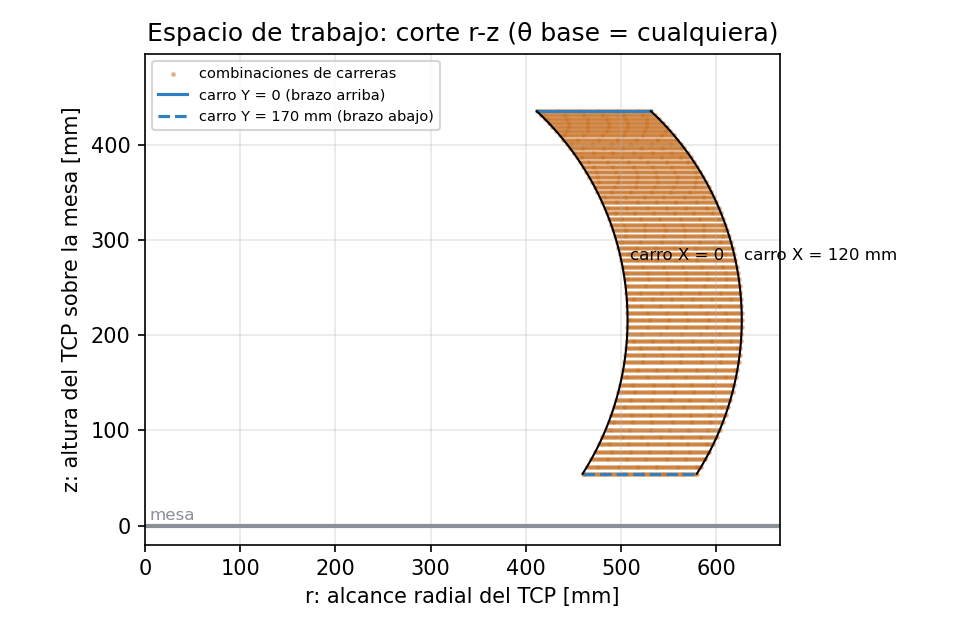
\includegraphics[width=\textwidth]{espacio_trabajo_rz.png}
\caption{Corte $r$--$z$.}\end{subfigure}
\begin{subfigure}{0.42\textwidth}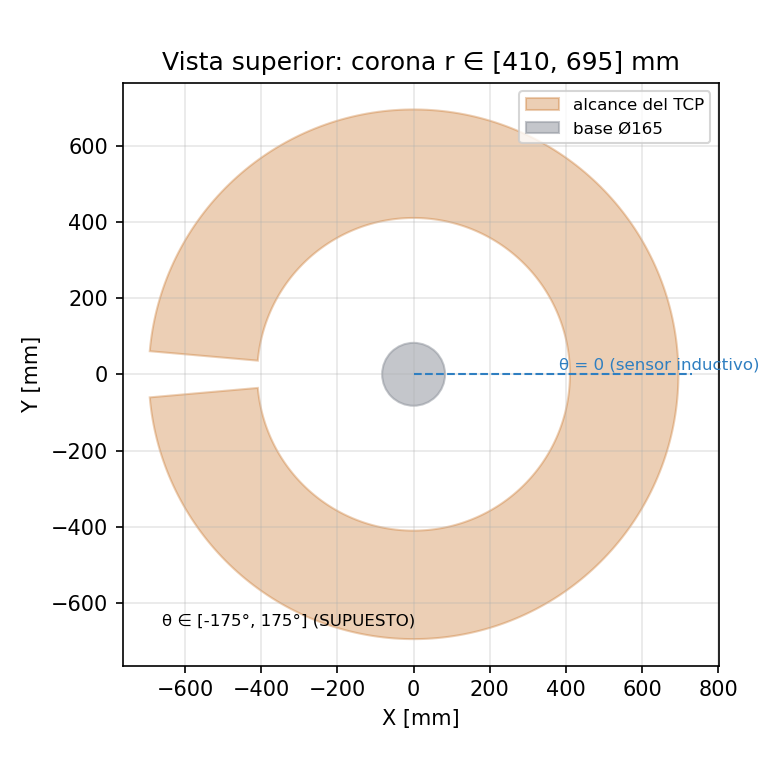
\includegraphics[width=\textwidth]{espacio_trabajo_superior.png}
\caption{Vista superior.}\end{subfigure}
\caption{Espacio de trabajo del TCP.}
\label{fig:espacio}
\end{figure}

El corte $r$--$z$ es la imagen del rectángulo de carreras $[0,120]\times[0,170]$. Los bordes $s_Y = $ constante son
segmentos horizontales, porque $s_X$ solo traslada en $r$. Los bordes $s_X = $ constante son arcos de radio
$L_9 = 300$ mm. El TCP alcanza $r \in [411, 627]$ mm y $z \in [54, 436]$ mm, unos 382 mm de recorrido
vertical. La ficha comercial del fabricante indica 0--400 mm en vertical y 0--120 mm adelante--atrás
\cite{ficha}, y el manual 440 mm para el eje Y. La diferencia se atribuye a los supuestos de la
tabla~\ref{tab:parametros}. En planta, el volumen es una corona de $\pm175°$.

%==================================================================== 11
\section{Modelo 3D y gemelo digital en la página}

\subsection{Modelo articulado a escala}
El GLB de trabajo (\codigo{brazo\_robotico\_v2.glb}) es una malla generada por IA y cortada en nodos. Su escala
es aproximada (la base mide 187 mm frente a los 165 mm reales) y los orígenes no están en los ejes, así que
se \textbf{rehízo de forma paramétrica}. El script \codigo{global/modelo-3d/generar\_modelo.js} (Node, sin
dependencias) construye cada pieza con primitivas a partir de las cotas de \codigo{web/js/cinematica.js} y
escribe el glTF binario. El resultado es \codigo{brazo\_xk-js1-1.glb}: 260 KB, 12 nodos y unos 3\,400
triángulos. Cada pieza móvil tiene el origen en su pivote o en su guía, y la jerarquía sigue el mecanismo:
\begin{lstlisting}
brazo_xk_js1_1
 +- base_fija
 +- base_giratoria   (R theta)
     +- carro_x      (P sX)
         +- carro_y  (P sY)
         |   +- biela_12   (R pasiva, pivote C)
         +- brazo_9        (R pasiva phi, pivote A)
         |   +- pinza      (R -phi: queda horizontal)
         |       +- mordaza_izq, mordaza_der (R eje vertical), tcp
         +- varilla_13     (R pasiva phi, pivote A')
\end{lstlisting}
Las bielas pasivas no se animan a mano: la página calcula sus ángulos con la cinemática directa.

\begin{figure}[H]
\centering
\begin{subfigure}{0.49\textwidth}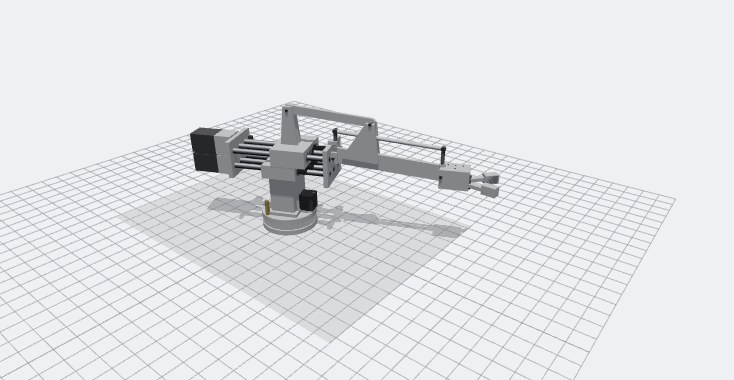
\includegraphics[width=\textwidth]{modelo_3d_isometrica.png}
\caption{Vista isométrica ($\theta=25°$).}\end{subfigure}
\begin{subfigure}{0.49\textwidth}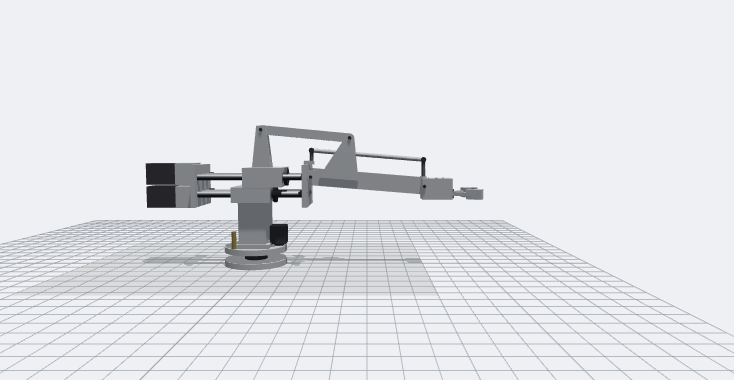
\includegraphics[width=\textwidth]{modelo_3d_lateral.png}
\caption{Vista lateral ($\theta=0$).}\end{subfigure}\\[4pt]
\begin{subfigure}{0.7\textwidth}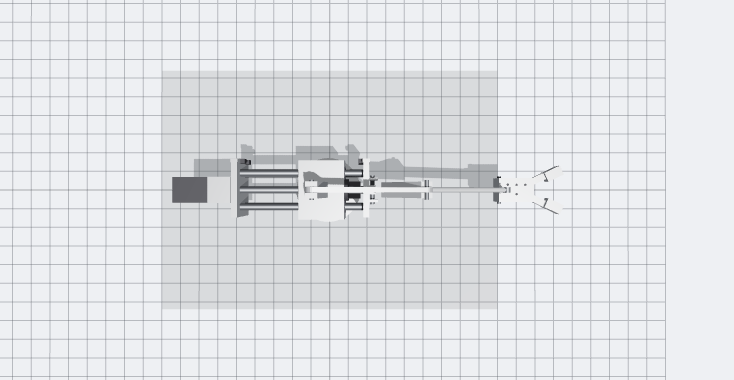
\includegraphics[width=\textwidth]{modelo_3d_superior.png}
\caption{Vista superior ($\theta=0$, $s_X = 40$, $s_Y = 130$ mm) sobre la mesa de 900 × 640 mm.}\end{subfigure}
\caption{Modelo 3D en el visor de la página ($s_X = 80$ mm, $s_Y = 120$ mm salvo indicación).}
\label{fig:modelo}
\end{figure}

\paragraph{Garra.} La garra tiene dos dedos planos que pivotan sobre ejes verticales en las esquinas
delanteras del cuerpo 4, de modo que \textbf{abren y cierran en el plano horizontal} (foto f18). En el modelo,
los nodos \codigo{mordaza\_izq} y \codigo{mordaza\_der} giran $\pm25°$ (\supuesto) con la garra abierta y
quedan paralelos con la garra cerrada (Q0.7 ON). El centro de los bloques de agarre coincide con el TCP.

\begin{figure}[H]
\centering
\begin{subfigure}{0.32\textwidth}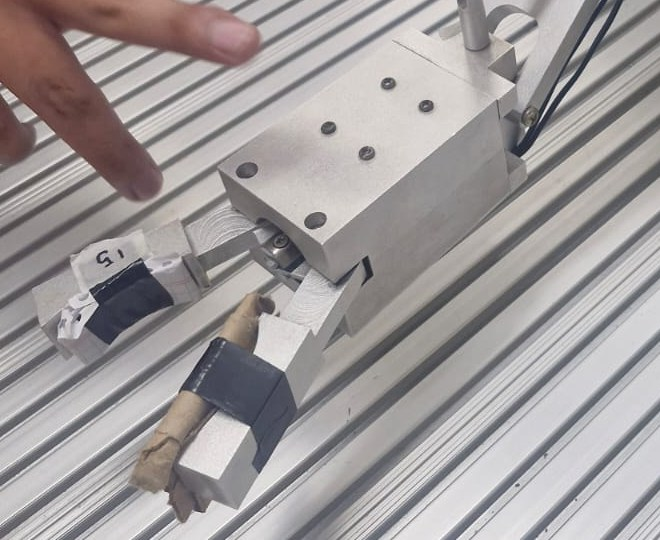
\includegraphics[width=\textwidth]{referencia_garra_f18.jpg}
\caption{Garra real (foto f18).}\end{subfigure}
\begin{subfigure}{0.32\textwidth}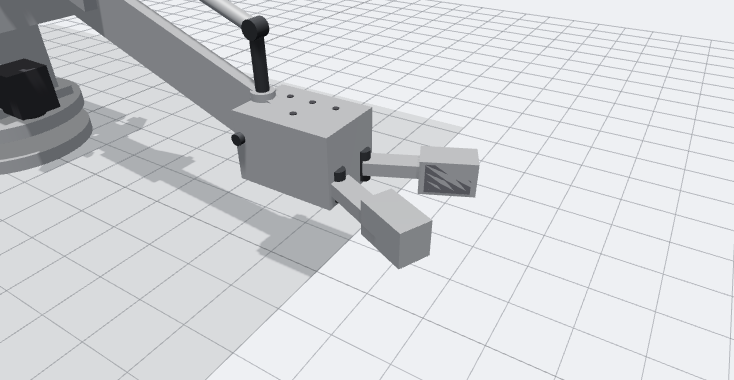
\includegraphics[width=\textwidth]{garra_abierta.png}
\caption{Modelo: abierta (Q0.7 OFF).}\end{subfigure}
\begin{subfigure}{0.32\textwidth}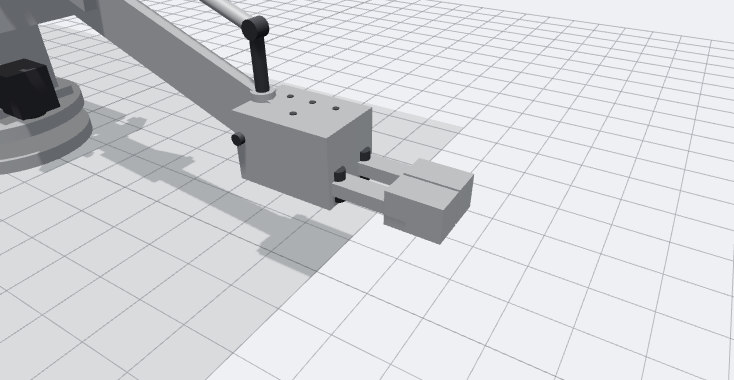
\includegraphics[width=\textwidth]{garra_cerrada.png}
\caption{Modelo: cerrada (Q0.7 ON).}\end{subfigure}
\caption{Garra de dedos horizontales.}
\label{fig:garra}
\end{figure}

\subsection{Sección ``Modelo 3D'' de la página}
La página (\url{https://brazo-4gdl.pages.dev}) incorpora:
\begin{itemize}
\item \textbf{Visor} three.js 0.160.0 con cámara orbital, vistas rápidas, mesa, rejilla y sombras suaves.
      Se carga en diferido, al llegar a la sección.
\item \textbf{Control articular} con deslizadores limitados a los recorridos y botón de garra.
\item \textbf{Control cartesiano}: la cinemática inversa mueve el modelo por una recta interpolada. Si un
      punto intermedio no es alcanzable, interpola en el espacio articular. Los objetivos inalcanzables se
      avisan con su motivo.
\item \textbf{Homing simulado}: carro Y a su final superior (I0.3), carro X al trasero (I0.1) y base hasta el
      sensor inductivo (I0.0), a velocidad reducida como recomienda el manual.
\item \textbf{Telemetría}: $\theta$, carreras, $\varphi$, pulsos por eje desde el origen, bits DIR, estado de
      I0.0--I0.4 y Q0.0--Q0.7, posición de la garra, $\det J$ y ángulo de transmisión.
\item \textbf{Secuencias pick \& place}: se graban puntos, se reproducen, se guardan en el navegador y se
      exportan en JSON y en CSV de pulsos y dirección por eje para programar el PLC.
\item \textbf{Indicadores} de límites, de colisión con la mesa y de movimiento simultáneo de X e Y, que el
      PTO compartido no permite.
\item \textbf{Módulo aislado} \codigo{web/js/conexion-plc.js} con \codigo{enviarPosicion()},
      \codigo{leerEstado()} y \codigo{homing()}. Hoy actúa sobre la simulación; en modo middleware habla
      por HTTP/JSON con la capa de aplicación de la arquitectura de 3 capas (Node-RED o Python), que es la
      que accede al S7-200.
\end{itemize}

%==================================================================== 12
\section{Validación}

\begin{table}[H]
\centering
\begin{tabular}{@{}lll@{}}
\toprule
\textbf{Prueba} & \textbf{Resultado} & \textbf{Criterio}\\
\midrule
Directa $\rightarrow$ inversa $\rightarrow$ directa (2205 puntos) & error $1.7\times10^{-13}$ & $<10^{-6}$\\
Jacobiano analítico frente a diferencias finitas & error $4.7\times10^{-8}$ & $<10^{-4}$\\
Pose del manual (fig. 1.3.3 A): pivotes $B$ y $C$ & $<5$ mm & foto de perfil\\
Python frente a JavaScript (25 puntos) & 0.05 mm & redondeo de la tabla\\
TCP del modelo 3D frente a la directa (visor) & $<10^{-13}$ mm & --\\
Lazo cerrado en todo el recorrido & sí & $90 \le d \le 380$ mm\\
Singularidades en el recorrido & ninguna & $|\det J| > 0$\\
\bottomrule
\end{tabular}
\caption{Validación numérica (\codigo{pruebas\_cinematica.js}, \codigo{graficas\_cinematica.py} y página).}
\end{table}

\begin{figure}[H]
\centering
\begin{subfigure}{0.49\textwidth}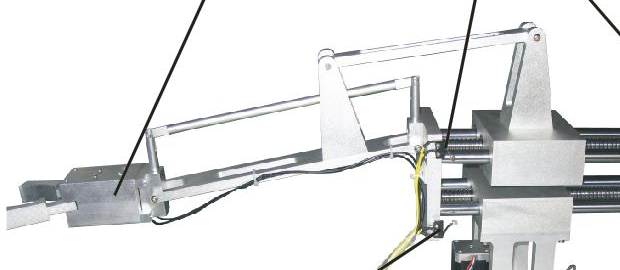
\includegraphics[width=\textwidth]{referencia_manual_perfil.png}
\caption{Foto de perfil del manual de fábrica.}\end{subfigure}
\begin{subfigure}{0.49\textwidth}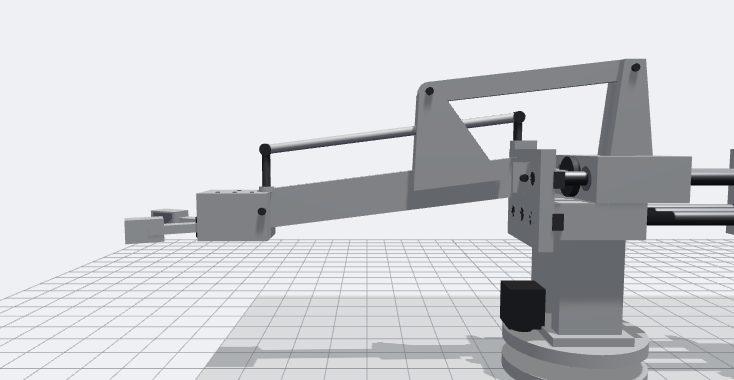
\includegraphics[width=\textwidth]{modelo_3d_pose_manual.png}
\caption{Modelo con $s_X = 0$, $s_Y = 125$ mm.}\end{subfigure}
\caption{Comparación cualitativa con la foto del manual: posición de la biela 12, la escuadra 8, la varilla 13
y la pinza. Las cotas estimadas se ajustaron con esta foto.}
\label{fig:comparacion}
\end{figure}

Con estas pruebas queda verificada la \textbf{consistencia interna}: las implementaciones coinciden entre
sí y con el modelo 3D. \textbf{Falta la validación contra la planta}, porque no se tuvo acceso a mover los
actuadores. Se propone el siguiente protocolo para el próximo laboratorio, compatible con las reglas de
seguridad de la Guía 4:
\begin{enumerate}
\item Hacer homing y llevar los carros a las 25 posiciones de \codigo{cinematica/tabla\_cinematica.csv}
      (combinaciones de $s_X \in \{0, 30, 60, 90, 120\}$ y $s_Y \in \{0, 42.5, 85, 127.5, 170\}$ mm, con sus pulsos).
\item En cada una, medir con flexómetro o escuadra la distancia horizontal del eje de giro al centro de las
      mordazas ($r$) y su altura sobre la mesa ($z$).
\item Comparar con la tabla. Ajustar primero el paso del husillo con el desplazamiento de $s_X$, luego $h_A$
      y $L_9$ con las alturas, y por último $a$ y $\beta$ con la curva $\varphi(s_Y)$.
\item Volver a ejecutar \codigo{pruebas\_cinematica.js}, \codigo{graficas\_cinematica.py} y
      \codigo{generar\_modelo.js}.
\end{enumerate}

\begin{table}[H]
\centering\small
\begin{tabular}{@{}rrrrrrr@{}}
\toprule
$s_X$ [mm] & $s_Y$ [mm] & $\varphi$ [°] & $r$ [mm] & $z$ [mm] & pulsos X & pulsos Y\\
\midrule
0 & 0 & 47.04 & 411.5 & 435.5 & 0 & 0\\
0 & 85 & 12.04 & 500.4 & 278.6 & 0 & 27200\\
0 & 170 & $-32.60$ & 459.7 & 54.4 & 0 & 54400\\
60 & 85 & 12.04 & 560.4 & 278.6 & 19200 & 27200\\
120 & 0 & 47.04 & 531.5 & 435.5 & 38400 & 0\\
120 & 127.5 & $-8.56$ & 623.7 & 171.3 & 38400 & 40800\\
120 & 170 & $-32.60$ & 579.7 & 54.4 & 38400 & 54400\\
\bottomrule
\end{tabular}
\caption{Extracto de la tabla de validación (posiciones previstas por el modelo).}
\end{table}

%==================================================================== 13
\section{Limitaciones}
\begin{itemize}
\item \textbf{Lazo abierto.} La posición de la garra es la \emph{estimada} a partir de los pulsos, no
      una medición. Si el motor pierde pasos por sobrecarga, aceleración excesiva o frecuencias altas (el par
      cae al 40--50~\% a la frecuencia máxima \cite{manual}), el modelo y la planta se separan y el error se
      acumula hasta el siguiente homing.
\item \textbf{Holguras.} Juego en los pasadores de las bielas, en los bujes lineales y en las tuercas de los
      husillos. El brazo amplifica el juego angular: un juego de 0.5° en $A$ desplaza el TCP
      $L_9 \cdot 0.5° \approx 2.6$ mm.
\item \textbf{Supuestos geométricos.} La posición de $A$ y $C$, $a$, $\beta$, $L_9$ y el TCP salen de
      estimaciones de foto. Un error de 5 mm en $h_A$ es un error de 5 mm en $z$. La validación del
      apartado anterior debe corregirlos.
\item \textbf{Transmisión supuesta.} Si el paso real fuera 10 mm/rev, todas las distancias calculadas a
      partir de pulsos se duplicarían. Medirlo es la prioridad número uno.
\item \textbf{Modelo solo cinemático.} No incluye masas, inercias ni la dinámica de los motores. Para el
      espacio de estados de la Guía 5 debe combinarse con la identificación del Laboratorio 4.
\item \textbf{Colisiones.} Solo se comprueba la mesa, no las colisiones entre piezas del propio brazo ni
      con objetos.
\end{itemize}

%==================================================================== 14
\section{Entregables de la guía vigente}
\label{sec:guia}
\begin{table}[H]
\centering
\begin{tabular}{@{}p{6.2cm}p{8.6cm}@{}}
\toprule
\textbf{Pide la Guía 5} & \textbf{Qué cubre este trabajo}\\
\midrule
Gemelo digital de la planta & Gemelo \emph{geométrico}: cinemática, modelo 3D y simulador web. Falta la dinámica identificada.\\
Archivos .m / .slx & \codigo{cinematica\_brazo.m} (directa, inversa, jacobiano, espacio de trabajo). No incluye Simulink.\\
Contraste con datos reales ($>$95~\%) & Protocolo y tabla de 25 puntos; queda pendiente medir en la planta.\\
Controlabilidad y observabilidad & No cubierto: requiere las matrices $A, B, C$ del Laboratorio 4.\\
Versionado en GitHub (ramas y merge) & Rama \codigo{feat/cinematica-modelo-3d}, con integración por pull request.\\
\bottomrule
\end{tabular}
\caption{Correspondencia con la Guía de Laboratorio N.º 5.}
\end{table}

%==================================================================== 15
\section{Conclusiones}

\subsection{Equipo de Control (ETN-902 / ETN-1034)}
\begin{itemize}
\item El XK-JS1-1 \textbf{no es un robot cartesiano}. El carro X traslada todo el brazo en dirección radial.
      El carro Y, a través de un mecanismo biela--manivela invertido, fija el ángulo del brazo y mueve la
      garra sobre un arco. Un paralelogramo mantiene la pinza horizontal. La movilidad en el plano es 2
      (Grübler), y con la base y la garra suma los 4 GDL del equipo.
\item La cinemática directa se reduce a cerrar un triángulo con la ley de cosenos. La inversa es analítica
      y, con la rama de montaje y los límites aplicados, da una solución única por cada $\theta$. No hay
      singularidades en el recorrido, y el ángulo de transmisión (38°--92°) es aceptable.
\item Con los supuestos actuales, la resolución es de 0.003 mm/pulso en los carros y 0.045 °/pulso en la
      base. Como $d\varphi/ds_Y \approx -0.45$ °/mm, un pulso del carro Y mueve el TCP unos 7.4 µm: la
      precisión real no la limitan los pulsos, sino las holguras y la pérdida de pasos.
\item El PTO compartido de la CPU 224 (Q0.1 con los relés K1 y K2) impide mover X e Y a la vez. Toda
      trayectoria programada en el PLC debe planificarse por turnos, y en una futura etapa de lazo cerrado
      convendría evaluar un módulo de posicionamiento o una CPU con más salidas PTO.
\item Quedan por medir el paso del husillo, los micropasos, la reducción de la base y los pivotes $A$ y
      $C$. La tabla de 25 puntos permite validar el modelo con un flexómetro.
\end{itemize}

\subsection{Equipo de Cómputo (ETN-1000)}
\begin{itemize}
\item La cinemática vive en un único módulo JavaScript sin dependencias (\codigo{web/js/cinematica.js}).
      Lo usan la página, el generador del modelo 3D y las pruebas, y exporta \codigo{parametros.json}
      para Python y MATLAB. Corregir una cota en ese archivo actualiza todo.
\item El modelo 3D se genera con un script reproducible, sin Blender: pesa 260 KB (el GLB de IA, 4.5 MB) y
      los orígenes de sus nodos están en los ejes reales.
\item El visor se carga en diferido y no frena el resto de la página. Funciona en escritorio y en
      celulares desde 375 px, en tema claro u oscuro, y sus controles se pueden usar con teclado.
\item \codigo{conexion-plc.js} define el contrato con el middleware: \codigo{POST /posicion},
      \codigo{GET /estado} y \codigo{POST /homing} en JSON. Es la pieza que conecta la página con la capa
      de aplicación y la base de datos de telemetría, donde se almacenan las posiciones estimadas.
\item Las secuencias exportadas en CSV (pulsos absolutos, incrementos y bits DIR por eje) pueden cargarse
      en la tabla de comandos de la base de datos y servir de entrada al programa del PLC.
\end{itemize}

%==================================================================== 16
\section{Recomendaciones}
\begin{itemize}
\item Medir el paso del husillo (10 vueltas), fotografiar los DIP de los drivers y contar los dientes del
      engranaje de la base.
\item Medir entre centros de pasadores las cotas $A$, $C$, $a$, $\beta$, $L_9$ y la posición del TCP.
\item Confirmar en la planta el mapa de E/S (I0.0 inductivo o final de carrera; Q0.5/Q0.6 como relés K1/K2).
\item Ejecutar el protocolo de validación y documentar el error de posición del gemelo.
\end{itemize}

%==================================================================== BIBLIOGRAFÍA
\begin{thebibliography}{9}
\bibitem{craig} J. J. Craig, \emph{Robótica}, 3.ª ed. México: Pearson Educación, 2006.
\bibitem{spong} M. W. Spong, S. Hutchinson y M. Vidyasagar, \emph{Robot Modeling and Control}. Hoboken: Wiley, 2006.
\bibitem{norton} R. L. Norton, \emph{Diseño de maquinaria}, 5.ª ed. México: McGraw-Hill, 2013.
\bibitem{manual} \emph{XK-JS1-1 Robotic Arm Training Device: Instruction Book} (manual de fábrica). Repositorio: \codigo{global/manuales/manual\_xk-js1-1\_en.pdf}.
\bibitem{s7200} Siemens AG, \emph{S7-200 Programmable Controller System Manual} y hoja de datos CPU 224 (6ES7214-1AD23-0XB0).
\bibitem{guia5} J. A. Nava, \emph{Guía de Laboratorio N.º 5}, ETN-902/ETN-1034/ETN-1000, UMSA, 2026.
\bibitem{ficha} Shandong Xingke Intelligent Technology Co., \emph{Educational Trainer, Robotic Arm Training Device (XK-JS1-1)}, ficha comercial. \url{https://www.china-manufacturer-directory.com/product/educational-trainer-robotic-arm-training-device-xk-js1-1_681727552.html}
\bibitem{gltf} Khronos Group, \emph{glTF 2.0 Specification}, 2021. \url{https://registry.khronos.org/glTF/}
\end{thebibliography}

\end{document}
